\section{Introduction}\label{sec:introduction}

\IEEEPARstart{H}{ybrid} ac/dc grids are increasingly operated through
voltage-source converters rather than through passive interfaces. Multi-terminal
dc links, offshore-wind collection systems, converter-interfaced generation,
and grid-forming resources make converter control limits part of the network
equilibrium itself. A converter may regulate active and reactive power, dc
voltage, or an internal ac voltage during normal operation, but semiconductor
current limits remain hard physical constraints. Once a limit becomes active,
the unconstrained command can no longer be maintained and the steady or
quasi-steady operating point changes control regime.

This limit-induced mode switching is more involved than the classical
generator PV/PQ transition. A converter can encounter an ac-current disk, a dc
power bound, saturated dc-voltage droop, and a selected priority between active
and reactive current. For a grid-forming converter, current limiting also
modifies the relation between the internal voltage source and the terminal
voltage. Consequently, a post-limit equilibrium may require explicit internal
voltage and current variables rather than a bus-level net-injection correction.
These issues are especially important in islanded networks, where a fixed GFM
internal phasor can provide the absolute angle reference without manufacturing
a terminal slack bus.

Unified hybrid ac/dc power-flow methods have improved the treatment of ac
networks, dc networks, and converter coupling
\cite{javid2023unified,sun2024mdhem,pompodakis2021generic}. In parallel, GFM
control and fault-current-limiting studies have clarified how a voltage-source
behavior is modified by current constraints
\cite{rocabert2012microgrid,baeckeland2022stationary}. Most power-flow
implementations nevertheless retain an external engineering loop of the form
``solve, inspect a limit, switch the device model, and solve again.'' This
approach is practical for isolated limits, but its equation dimension,
variable semantics, and sparse pattern may depend on the switching sequence.
Simultaneous activation, priority ties, and return switching can also make the
final result sensitive to implementation order.

Complementarity equations provide a fixed-dimensional alternative. A limit
and its multiplier are solved together, allowing the inactive and active
regimes to be represented by one nonsmooth system
\cite{facchinei2003complementarity,fischer1992newton}. Semismooth Newton
methods can then achieve fast local convergence without enumerating all mode
combinations \cite{qi1993nonsmooth}. Their use in a production hybrid ac/dc
solver, however, raises three additional questions. First, the converter must
own explicit local variables so that device equations and result certificates
do not have to be reconstructed from aggregated bus injections. Second, the
fixed equation layout must translate into a measurable sparse-linear-algebra
advantage rather than only a software convenience. Third, local convergence
claims must distinguish a numerically accepted generalized-Jacobian element
from the stronger BD-regularity condition over the B-subdifferential.

This paper addresses these questions through a balanced positive-sequence
hybrid ac/dc formulation with explicit converter blocks. Each supported VSC
owns the local state
\begin{equation}
 z_c=(P_{\ac,c},Q_{\ac,c},P_{\dc,c},E_{r,c},E_{i,c},\lambda_c),
 \label{eq:local-state-intro}
\end{equation}
where the internal-voltage slots are active for GFM operation and are fixed by
identity equations for power-port modes. Current-magnitude scaling uses a
Fischer--Burmeister equation. Active- and reactive-power priorities use nested
median projections. Vdc-Q operation includes a saturated dc-voltage droop
command, and GFM operation uses an internal voltage behind virtual impedance.
All equations remain present across limit activation.

The main contributions are as follows.

\begin{enumerate}
  \item A unified fixed-dimensional converter-limit model is developed for
  PQ, Vdc-Q, and GFM operation. It combines the ac-current disk, magnitude or
  P/Q priority, converter energy balance, saturated dc-voltage droop, and GFM
  Norton equations while preserving stable device identity and explicit local
  result variables.

  \item A production semismooth Newton method is formulated with analytic
  network/local generalized Jacobians. Exact Fischer--Burmeister and median
  equations define the reported root; optional Kanzow/CHKS smoothing provides
  a fixed-pattern continuation for difficult degenerate points. A full sparse
  Newton fallback remains available at every iteration.

  \item An exact local-block Schur method eliminates all six-state converter
  blocks before network factorization. The method has $O(m)$ local dense work
  for $m$ converters, removes exactly $6m$ unknowns, and reduces the assembled
  structural nonzeros by at least $48m$ under the stated three-port coupling
  pattern. Local reciprocal-condition and normwise backward-error tests guard
  the reduced and reconstructed full steps.

  \item The convergence statement separates mathematics from runtime
  evidence. BD-regularity plus semismoothness yields local superlinear
  convergence, and strong semismoothness yields the standard quadratic rate.
  Runtime certificates establish nonsingularity and backward stability only
  for the selected generalized-Jacobian element; they are not presented as a
  proof over every element of the B-subdifferential.

  \item The implementation is exercised through registered production tests,
  OpenDSS circuit validation, OPF-to-PF replay, transient Norton initialization,
  simultaneous limits, weak-grid and infeasible cases, GFM islands, and real
  hybrid case300/ACTIVSg2000 benchmarks. The preliminary results also retain a
  negative small-system performance result, which motivates an explicit and
  configurable production admission rule.
\end{enumerate}

Figure~\ref{fig:problem-method} summarizes the problem, model ownership, and
solver structure. The central distinction is that limit activation changes
residual values and generalized derivatives, but not the converter state,
equation coordinates, or sparse ownership map.

\begin{figure*}[t]
\centering
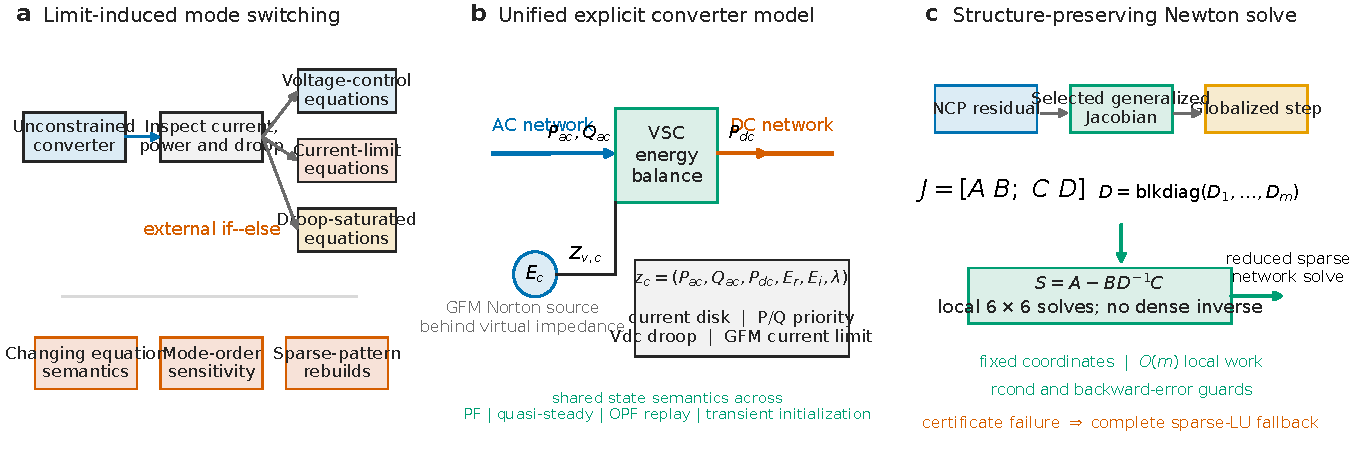
\includegraphics[width=\textwidth]{figures/problem_method_overview.pdf}
\caption{From limit-induced switching to the proposed fixed-dimensional
framework. (a) External mode switching can change equation semantics and
sparse structure. (b) Each VSC instead owns one explicit six-state block,
including the GFM internal voltage behind virtual impedance. (c) The resulting
fixed generalized-Jacobian pattern supports certified local-block Schur
elimination with complete sparse-LU fallback.}
\label{fig:problem-method}
\end{figure*}

The paper is organized as follows. Section~\ref{sec:model} defines the network
and converter equations. Section~\ref{sec:ssn} presents the semismooth Newton
method. Section~\ref{sec:schur} derives the exact local-block Schur elimination
and its cost. Section~\ref{sec:convergence} states the regularity and local-rate
conditions. Section~\ref{sec:preliminary} reports the current production
evidence and its limitations.
